\documentclass{article}
\usepackage[nl]{../personal-packages/thomas/packages/mathy}
\usepackage{kvoptions}
\usetikzlibrary{matrix}

\begin{document}
    \tableofcontents
    \newpage

    \section{Binomiaalco\"efficienten}\label{sec:binomiaalco"efficienten}

    \[
        \binom n k = \frac{n!}{k! (n-k)!} = \frac{n! / (n-k)!}{k!} = \frac{n (n-1) \dots (n-k+1)}{k!}.
    \]
    Merk op dat we voor $n$ ook negatieve en niet-gehele getallen in kunnen vullen als we maar de goede (meest rechtse) definitie gebruiken.

    \section{Limieten}\label{sec:limieten}
    Onthoud
    \begin{align*}
        &\lim_{x\to 0} \frac{x}{\sin x} = 1 \\
        &\lim_{n \to \infty} \left( 1 + \frac a n \right)^n = e^a \\
        &\lim_{n \to \infty} \sqrt[n]{n} = 1 \\
    \end{align*}
    \[
        f(h) \in o(h) \text{ als } \lim_{h \downarrow 0} \frac{f(h)}{h} = 0.
    \]
    \section{Machtreeksen}\label{sec:sommen}
    \input{sommen}

    \section{Taylorreeksen}\label{sec:taylorreeksen}
    \input{taylorreeksen}

    \section{Integralen}\label{sec:integralen}

    \begin{stelling}[Bell curve]
        \[ \int_{-\infty}^\infty e^{-\alpha x^2} \d x = \sqrt {\frac \pi \alpha}.\]
    \end{stelling}

    \begin{stelling}[Limiet door de integraal halen]
        Zij $\f_k,\f \: \reals^n \to \reals$, met $\lim_{k \to \infty} \f_k = \f$, dan
        \[ \f_k \text { \textbf{convergeert uniform} naar } \f \implies \lim \int \f_k = \int \lim \f_k = \int \f \,. \]
    \end{stelling}

    \section{Integreren}\label{sec:integreren}
    \input{integreren}

    \section{Afgeleides}\label{sec:afgeleides}
    \subsection{Afgeleide van $z^x$}\label{subsec:afgeleide-van}
    \[
        \frac{\d}{\d x} z^x = \frac{\d}{\d x} e^{\log \left( z^x \right)} = \frac{\d}{\d x} e^{x \log z} = \log z e^{x \log z} = z^x \log z.
    \]

    \section{Co\"ordinaten}\label{sec:coordinaten}
    \input{coordinaten}

    \section{Momenten uitrekenen}\label{sec:momenten-uitrekenen}
    \input{momenten}

    \section{Matrices en vectoren}\label{sec:matrices-en-vectoren}
    \subsection{Inverse $2 \times 2$ matrix}\label{subsec:inverse-2x2-matrix}
\[
    A = \matrix{a & b \\ c & d} \implies A^{-1} = \frac{1}{\mathrm{det} A} \matrix{d & -b \\ -c & a} = \frac{1}{ad-bc} \matrix{d & -b \\ -c & a}.
\]
Je kunt controleren of je $-a$ en $-d$ of $-b$ en $-c$ moest nemen door $\matrix{1&0\\0&1}=I=I^{-1}$ in te vullen.

\subsection{Inverse $n \times n$ matrix}
Veeg
\[
    [A|I] \sim \dots \sim [I|A^{-1}].
\]

$A$ is non-singulier $\iff$ $|A|=\Pi_i \lambda_i \neq 0$ $\iff$ A heeft een inverse.

\subsection{Determinant}\label{sec:determinant}
\input{determinant}

\subsection{Inproduct/uitproduct}\label{sec:inproduct/uitproduct}
\paragraph{Inproduct (dot product)}
\[
    \x \bullet \bm \phi = \matrix{x \\ y \\ z} \bullet \matrix{\phi_1 \\ \phi_2 \\\phi_3} = x \phi_1 + y \phi_2 + z \phi_3
\]
\[
    a \bullet b = \abs a \abs b \cos(a, b)
\]

\paragraph{Uitproduct (Vector/Cross product)}
\[
    \matrix{x \\ y \\ z} \times \matrix{\phi_1 \\ \phi_2 \\\phi_3} = \matrix{y \phi_3 - \phi_2 z \\ z \phi_1 - \phi_3 x \\ x \phi_2 - \phi_1 y}
\]
eventueel te onthouden door (zie \LaTeX\ comments)
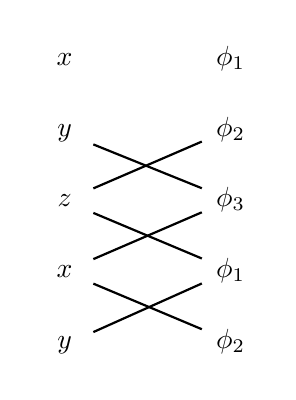
\begin{tikzpicture}[thick]
    \matrix (m) [matrix of math nodes, row sep = 1em, column sep = 4 em, minimum width=2em]
    {
        x & \phi_1 \\
        y & \phi_2 \\
        z & \phi_3 \\
        x & \phi_1 \\
        y & \phi_2 \\
    };
    \path[-stealth]
    (m-2-1) edge[-] (m-3-2) % y keer phi_3
    (m-2-2) edge[-] (m-3-1) % min phi_2 keer z,
    (m-3-1) edge[-] (m-4-2) % z keer phi_1
    (m-3-2) edge[-] (m-4-1) % min phi_3 keer x,
    (m-4-1) edge[-] (m-5-2) % x keer phi_2
    (m-4-2) edge[-] (m-5-1) % min phi_1 keer y
    ;
\end{tikzpicture}

\subsection{Eigenwaarden en eigenvectoren}

Voor matrix $A$, eigenwaarde $\lambda$ en bijbehorende eigenvector $v$, moet gelden $Av = \lambda v$.
De eigenwaarden zijn de nulpunten van het karakteristieke polynoom $|A - \lambda I|$.
Bijvoorbeeld voor $A = \matrix{a & b \\ c & d}$, krijgen we $(a - \lambda)(d - \lambda) - bc = 0$.
% todo eigenvectors

    \section{Inhoud bol}\label{sec:inhoudBol}
    \input{inhoud-bol}

    \section{Tussenwaarde/middelwaardestelling}\label{sec:tussenwaarde/middelwaardestelling}
    \begin{stelling}[\indx{Tussenwaardestelling}/Intermediate Value Theorem]

        Zij $a,b \in \reals,\ a<b,\
            f:[a,b]\to \reals \text{ continu}\,.
        $
        Zij $f(a)<y<f(b)$.
        Dan \[ \exists_{c\in(a,b)}:f(c)=y. \]
    \end{stelling}

    \begin{stelling}[\indx{Middelwaardestelling}/Mean Value Theorem]

        Zij $f\:[a,b] \to \reals$ continu, $f|_{(a,b)}$ differentieerbaar.
        Dan
        \[
            \exists_{c \in (a,b)} : f'(c) = \frac{f(b)-b(a)}{b-a}\,.
        \]
    \end{stelling}

    \section{Kwadraat afsplitsen}\label{sec:kwadraatAfsplitsen}
    Om een kwadratische vergelijking $x^2 + ax + b = 0$ op te lossen voor $x$ kunnen we in plaats van de abc-formule ook kwadraat afsplitsen.
    Let wel op dat de co\"efficient voor de $x^2$ een 1 is.
    \begin{align*}
        x^2 + a x + b &= 0 \\
        \left(x + \frac{1}{2} a\right)^2 - \left( \frac{1}{2}a \right)^2 &= - b \\
        \left(x + \frac{1}{2} a\right)^2 &= \left( \frac{1}{2}a \right)^2 - b \\
        x + \frac{1}{2} a &= \pm \sqrt{\left( \frac{1}{2}a \right)^2 - b} \\
        x &= -  \frac{1}{2} a \pm \sqrt{\left(\frac{1}{2}a \right)^2 - b}
    \end{align*}

    \newpage
    \section{Appendix}\label{sec:appendix}
    \begin{lstlisting}{language=mathematica}
        (* Transparent sphere *)
        pp = ParametricPlot3D[
        {Cos[u] Sin[v],
        Sin[u] Sin[v],
        Cos[v]},
        {u, 0, 2 Pi}, {v, 0, Pi}, Boxed -> False, Axes -> False,
        PlotStyle -> Opacity[0.05]];
        (* Part on the sphere (hold r) *)
        pp1 = ParametricPlot3D[
        {Cos[u] Sin[v],
        Sin[u] Sin[v],
        Cos[v]},
        {u, 0, 2 Pi}, {v, 0, Pi/6}, Axes -> False, Boxed -> False];
        (* Cone (hold v) *)
        pp2 = ParametricPlot3D[
        {r Cos[u] Sin[Pi/6],
        r Sin[u] Sin[Pi/6],
        r Cos[Pi/6]},
        {r, 0, 1}, {u, 0, 2 Pi}, Axes -> False, Boxed -> False];
        (* Combine the three parts *)
        Show[pp, pp1, pp2, ImageSize -> Large]
    \end{lstlisting}
    \begin{figure}[h!]
        \centering
        \includegraphics[width=.5\textwidth]{bol.png}
        \caption{Bol in Mathematica}\label{bolMMa}
    \end{figure}
\end{document}